\documentclass{ximera}
\usepackage{tikz}
\usepackage{color}
\usepackage{amsmath,amssymb,amsfonts}
\usepackage{graphicx}
%\usepackage{helvet}
%\renewcommand{\familydefault}{\sfdefault}
\author{Jeffrey Kuan}
\input{../preamble} %% Loads the graphics path
\title{An example webpage}
\license{CC: 0}
\begin{document}

\begin{abstract}
   I like Taylor Swift.
\end{abstract}
\maketitle
%\part{Introduction}
%\chapterstyle
%    \activity{basics/basicWorksheet}
%    \sectionstyle
%    \activity{basics/exercises/someExercises}

%    \chapterstyle
%    \activity{basics/graphicsInteractives}

Accessibility statement: This webpage is WCAG2.1AA compliant, and I tested out this webpage on NVDA. 
You can also \href{https://ximera.osu.edu/firststeps24html/aFirstStepInXimera/basics/MAA_AMS_Example.tex}{download the TeX source file.}

\section{About this webpage}
This webpage was created with \href{https://ximera.osu.edu/}{Ximera}, an 
interactive textbook platform hosted by Ohio State University. The Ximera Project is funded 2024-2026 (with no other external funding) by a 
\$2,125,000 \href{https://www.ed.gov/grants-and-programs/grants-higher-education/improvement-postsecondary-education/open-textbooks-pilot-program}{Open Textbooks Pilot Program} grant from the federal Department of Education.



\section{An example of alternative text}

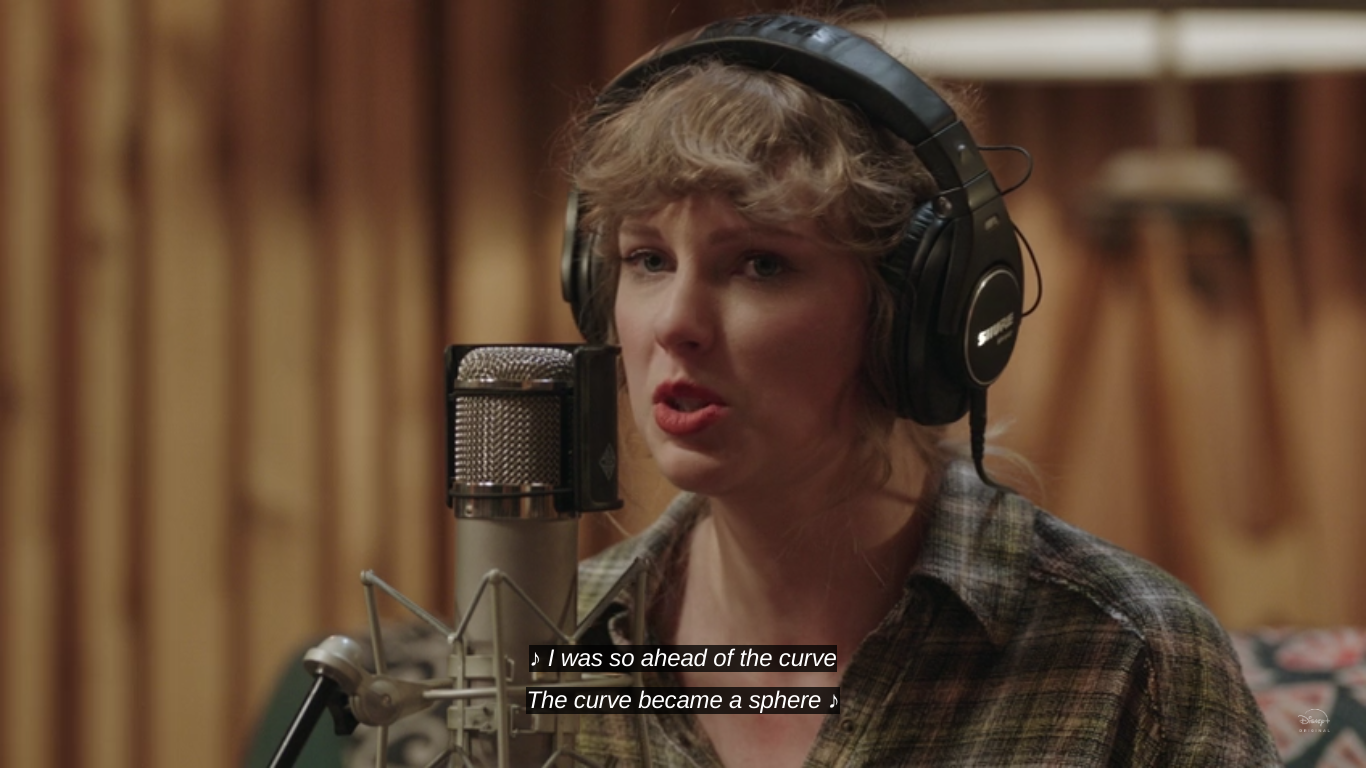
\includegraphics[alt={Taylor Swift in front of a microphone and wearing headphones. There are captions that read 'I was so ahead of the curve, the curve became a sphere'}]{TaylorSwiftScreenshot.png}




\begin{thebibliography}{10}

\bibitem{FRT88} L. D. Faddeev, N. Yu. Reshetikhin, L. A. Takhtajan, Quantization
of Lie groups and Lie algebras, Algebraic analysis, Vol. I, Academic
Press, Boston, MA, (1988), 129-139.

\end{thebibliography}

\end{document}